\subsection{Side muon range detector}
Two Side-MRD modules will be constructed by the end of January 2018. 
Each Side-MRD module is composed of iron plates and scintillator bars for tracking secondary particles from neutrino interactions.
Support structure of the Side-MRD module mainly consists of 11 steel plates of which dimensions are $1800\times1610\times30$ mm$^{3}$, is sized as $2236\times1630\times975$ mm$^{3}$ as shown in Fig. \ref{fig:side_mrd_support_structure}, and weights $\sim$8.5 ton. 
Scintillator bars were produced by Uniplast company in Vladimir, Russia. Each bar is polystyrene based and made by extrusion technology with scintillating composition of 1.5\% PTP and 0.01\% POPOP. Then each bar's suface is etched by a cemical agent to form a white diffuse layer. The usage of this method gives almost ideal contact between the scintillator and the reflector which allows us to gain in light yield up to 50\% compared to clear scintillator. 80 scintillator bars are installed in one Side-MRD module, and each scintillator bar is sized as $1800\times200\times7$ mm$^{3}$ including reflector part. 
Scintillation light is collected by wave length shifting fibers, Y-11 (S type) with a diameter of 1.0 mm produced by Kuraray. 
The fiber is glued by optical cement EJ-500 in a S-shape groove on the surface of the scintillator bar as shown in Fig. \ref{fig:side_mrd_scintillator}. Using this technique allows us to uniform light collection over scintillator's sufaces.
Two optical connectors as shown in Fig. \ref{fig:side_mrd_optical_con} are attached to either end of the fiber, and scintillation light is lead to two MPPCs, S13081-050CS(X1), produced at Hamamatsu Photonics. Optical connector of such type (so-called Baby-mind type of optical connector) consists of two parts (see Fig. \ref{fig:side_mrd_optical_con}): a) a MPPC cover and b) a ferrule. Ferrule b) is fixed in scitillator by glue with glued fiber in it, cut by mill and polished to form an optical contact between the fiber end and the MPPC. Cover a) is clicked into place on ferrule b) and used to fix MPPC in optical contact. To ensure the tightness of the contact between the MPPC window and the fiber's end in ferrule a special spring made of sponge rubber is used (Fig. \ref{fig:side_mrd_optical_scheme}). 
For each MPPC, 667 pixels of APD are aligned in a shape of square 1.3 mm on a side. 

\begin{figure}[tbh]
\begin{center}
\includegraphics[width=0.8\linewidth]{fig/side_mrd_structure.pdf}
\end{center}
\caption{
Support structure of the Side-MRD module.
}
\label{fig:side_mrd_support_structure}
\end{figure}

\begin{figure}[tbh]
\begin{center}
\includegraphics[width=0.8\linewidth]{fig/side_mrd_scintillator.pdf}
\end{center}
\caption{
Scintillator bar of the Side-MRD modules.
}
\label{fig:side_mrd_scintillator}
\end{figure}

\begin{figure}[tbh]
\begin{center}
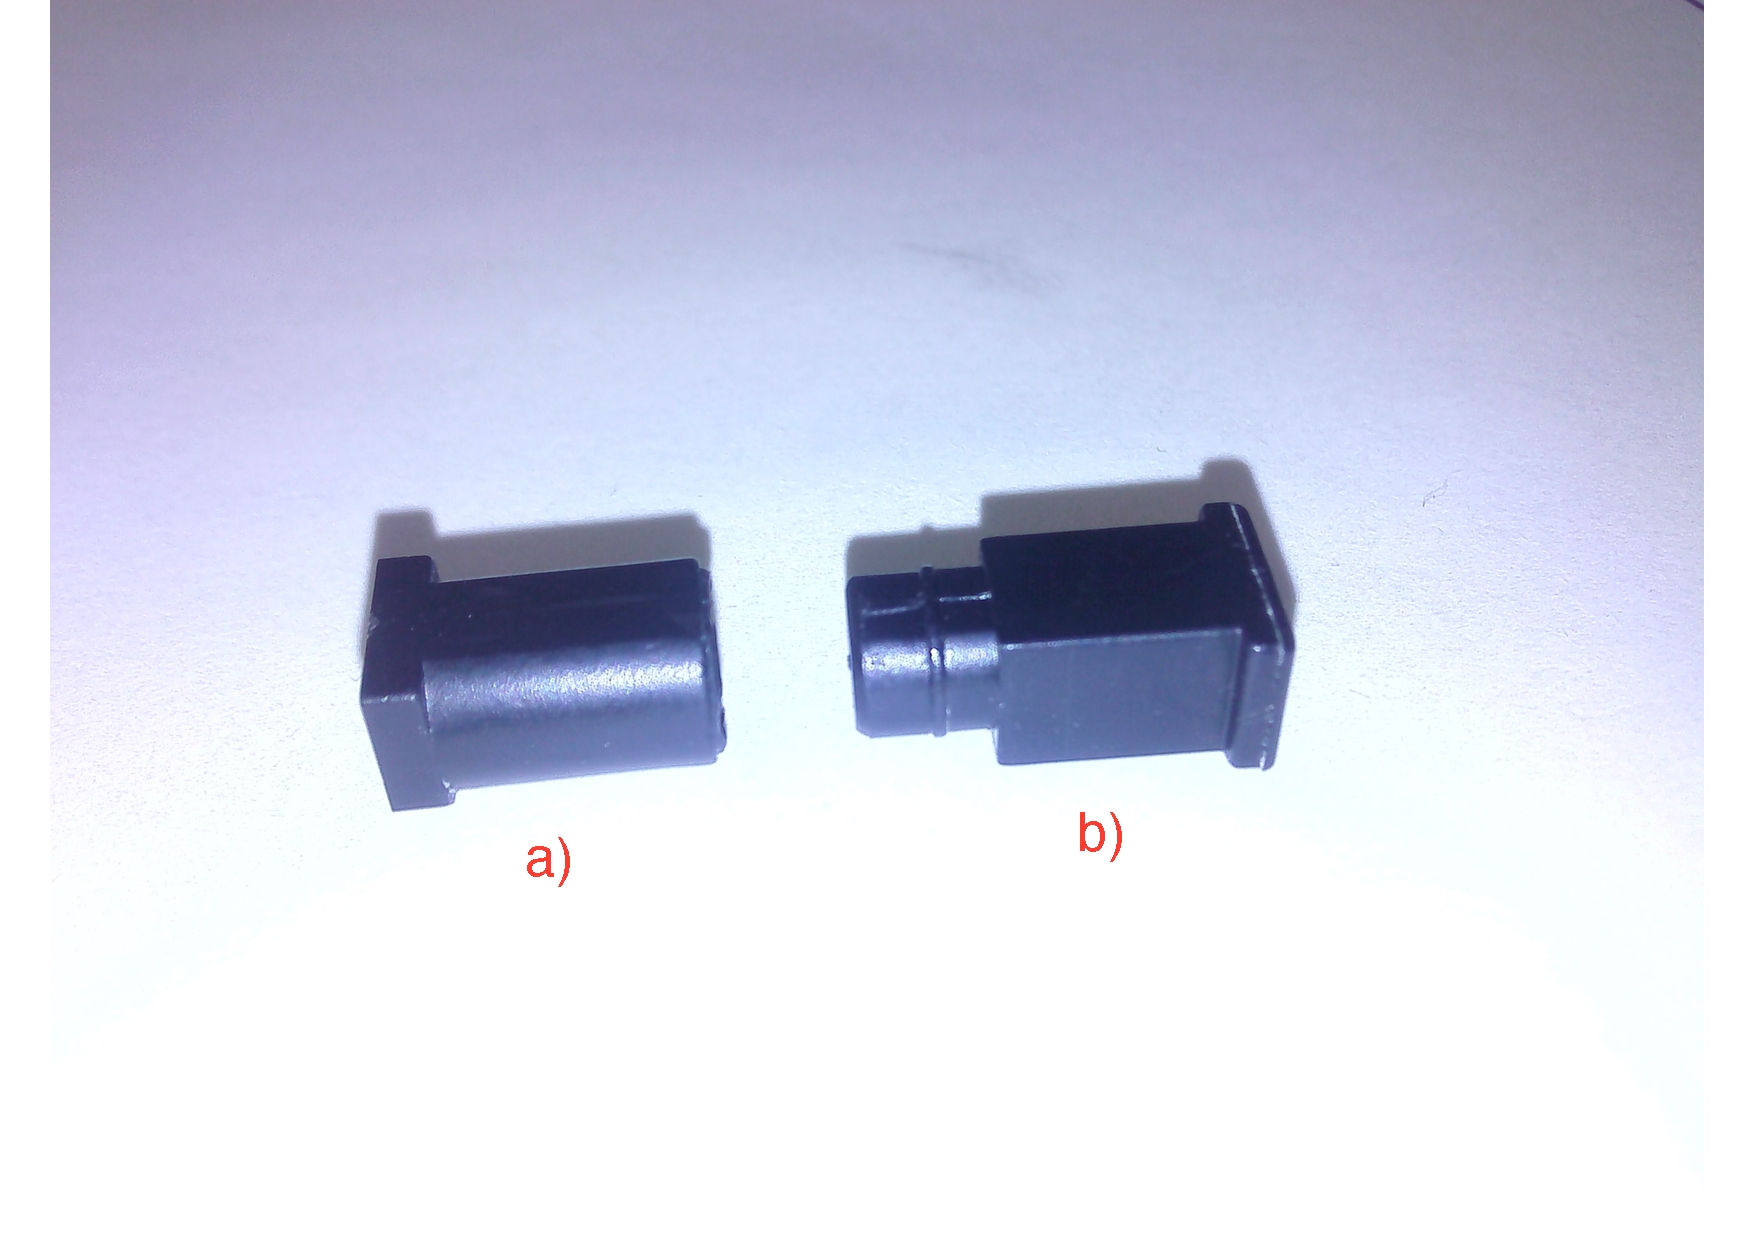
\includegraphics[width=0.8\linewidth]{fig/side_mrd_optical_con.pdf}
\end{center}
\caption{
Optical connector for the Side-MRD scintillator. a) MPPC cover. b) Ferrule.
}
\label{fig:side_mrd_optical_con}
\end{figure}

\begin{figure}[tbh]
\begin{center}
\includegraphics[width=0.8\linewidth]{fig/side_mrd_optical_scheme.pdf}
\end{center}
\caption{
Scheme of the MPPC placement in optical connector.  a) MPPC cover. b) Ferrule. c) Spring (sponge rubber). d) MPPC.
}
\label{fig:side_mrd_optical_scheme}
\end{figure}

Construction of scintillator bars of the Side-MRD modules had been completed at INR in Russia, and they were transported to Japan in July 2017. Before and after the shipping their perfomance were check with cosmic rays. The main mesured parameters were light yield and light yield assymetry. For the light yields $LY_{1}$ and $LY_{2}$ at counter's two ends correspondent assymetry is calculated as $100\% \times \frac{LY_{1}-LY_{2}}{LY_{1}+LY_{2}}$. Thus at INR we selected 324 counters from total 332 produced with mean light yield of 45 p.e./MIP and assymetry less than 10 \% at the center of the bar. When counters arrived to Japan their perfomance were checked once again at Yokohama National University. In the bench setup here two small trigger counters were put in the center of measured bars. Trigger signal is the coincidence between top and buttom trigger counters made of $NaI (Tl)$ crystals of $6 \times 6 \times 17 cm^{3}$ size. Average total light yield obtained in the central part of the scintillator slab is 40 p.e./MIP and varies from 32 to 50 p.e/MIP. (Fig. \ref{fig:side_mrd_ly} (left)). Only two counters here showed relatively high assymetry close to 25 \% as shown in Fig. \ref{fig:side_mrd_ly} (right). By such quality assurance tests of the counters we selected 320 scintillator bars to be installed in four Side-MRD modules. In addition, for four counters there were measured time resolution for single and combination of the counters. For one counter time resolution defined as uncertanty on $(T_{left}-T{right})/2$ was obtained $\sigma$ = 1ns (Upper left plot in Fig. \ref{fig:side_mrd_combi_time}). Further, for a set of $n$ counters combined time resolution will be $\frac{(T_{L}-T_{R})_{1}+(T_{L}-T_{R})_{2}+...+(T_{L}-T_{R})_{n}}{2 \times n}$. The result of combination of 2,3,4 counters is 0.79 ns, 0.66 ns and 0.68 ns accordingly (Fig. \ref{fig:side_mrd_combi_time}).  
\begin{figure}[tbh]
\begin{center}
\includegraphics[width=0.8\linewidth]{fig/side_mrd_ly.pdf}
\end{center}
\caption{
Total light yield distribution (left) and light yield assymetry (right) measured at YNU.
}
\label{fig:side_mrd_ly}
\end{figure}

\begin{figure}[tbh]
\begin{center}
\includegraphics[width=0.8\linewidth]{fig/side_mrd_combi_time.pdf}
\end{center}
\caption{
Time resolution for one (upper left) and a set of 2,3,4 Side-MRD counters.
}
\label{fig:side_mrd_combi_time}
\end{figure}
Construction of Side-MRD modules will be done from November 2017 to January 2018 at Yokohama National University, then they will be transported to J-PARC and will be installed to the B2 floor of the T2K near detector hall before staring the T2K beam in March 2018.
